\section{Conclusion}

\makesection{
\notes{
\begin{itemize}
\item I will now recap the contributions of my framework.
\end{itemize}
}
{
\begin{itemize}
\item recap contributions
\end{itemize}
}
}

\subsection{Contributions}

\begin{frame}{Conclusion}

\begin{itemize}
\item Less involvement is required from the user
\item Versatile matching procedure
\item Proof generation
\item Rich language
\end{itemize}

\notes{
\begin{itemize}
\item Firstly, the framework provides a more expressive and dynamic way of writing proofs.
\item This is partly thanks to the proposed matching procedure which has inference capabilities, and can be applied to different use cases.
\item This framework ultimately generates LISA proofs that can be checked for correctness, exported or even imported.
\item Finally the rich and expressive languages simplifies the usage of this system.
\end{itemize}
}
{
\begin{itemize}
\item firstly, more expressive and dynamic
\item thanks to matching, inference, different use cases
\item only LISA trusted
\item rich language improves usability
\end{itemize}
}

\end{frame}

\subsection{References}

\begin{frame}{Material}

\centering

Source code: \href{https://github.com/FlorianCassayre/master-project}{\code{github.com/FlorianCassayre/master-project}}

\vspace{0.5cm}

\begin{tikzpicture}[image/.style={inner sep=0.3mm,outer sep=0,draw=none,shade,top color=gray,bottom color=gray,blur shadow={shadow blur steps=10}}]

\node[image] (e) [xshift=8cm, yshift=0cm] {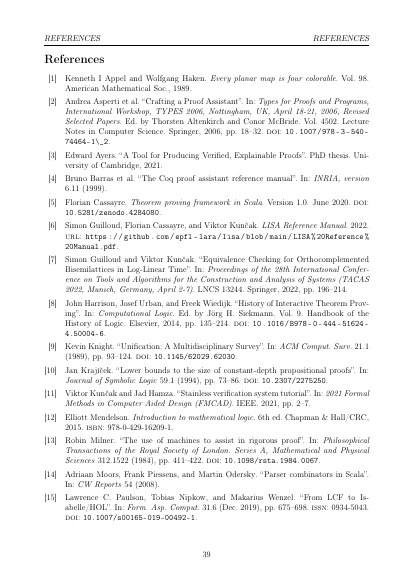
\includegraphics[height=4cm]{figures/thumbnail-39.png}};
\node[image] (d) [xshift=6cm, yshift=-0.5cm] {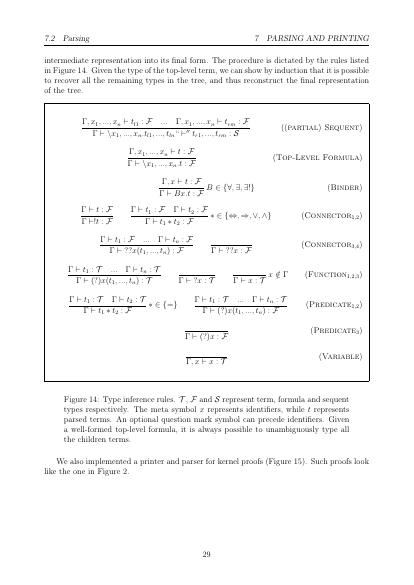
\includegraphics[height=4cm]{figures/thumbnail-29.png}};
\node[image] (c) [xshift=4cm, yshift=0cm] {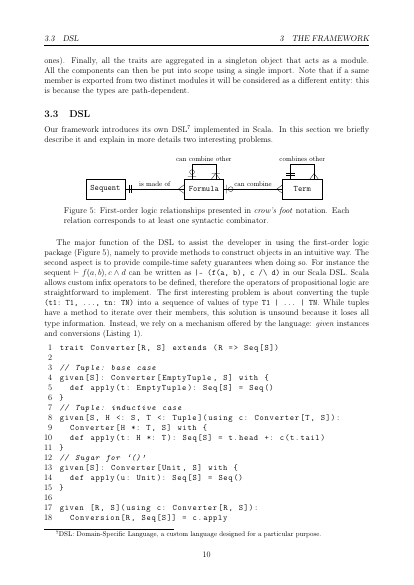
\includegraphics[height=4cm]{figures/thumbnail-10.png}};
\node[image] (b) [xshift=2cm, yshift=-0.5cm] {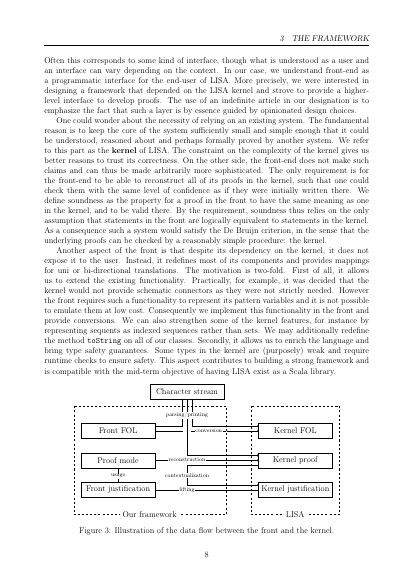
\includegraphics[height=4cm]{figures/thumbnail-08.png}};
\node[image] (a) {
\includegraphics[height=4cm]{figures/thumbnail-01.png}};
\end{tikzpicture}

\vspace{0.5cm}

\href{https://zenodo.org/record/6645113}{\code{doi:10.5281/zenodo.6645113}}

\notes{
\begin{itemize}
\item The source code along with the thesis report is published on Zenodo.
\item Thank you very much for your attention. The first part of this presentation is over, I will now be taking and answering questions from the audience.
\end{itemize}
}
{
\begin{itemize}
\item source code and report on Zenodo
\item thanks; questions
\end{itemize}
}

\end{frame}
